\documentclass[a4paper,11pt,headings=standardclasses,parskip=half]{scrartcl}

% font, style, etc.
\usepackage[utf8]{inputenc} % defines
\usepackage{csquotes}
\usepackage{xspace} % proper space after macros with 0 args

% mathematics
\usepackage{amsmath}
\usepackage{amssymb}

% figures, tables, etc.
\usepackage{hyperref} %
\usepackage{graphicx}
\usepackage{tikz}
\usepackage{pgf}
\usepackage{xcolor}
\usepackage{placeins} % -> floatbarrier
\usepackage{siunitx}  % -> handling of units
\usepackage[printwatermark]{xwatermark}
\newwatermark[allpages, color=red!50,angle=45,scale=1.8,xpos=0,ypos=0]{\textsf{DRAFT ONLY, NOT APPROVED}}

% code
\usepackage{listings}
\lstset{
language=Python, 
backgroundcolor = \color{light-gray},
basicstyle=\scriptsize\sffamily,
stringstyle=\color{orange},
breaklines=true,
numberstyle=\tiny\color{gray},
keywordstyle=\bfseries\color{dark-blue}\textit, % print keywords dark-blue
commentstyle=\color{dark-green}, % print comments dark-green
showstringspaces=false} % spacing between strings not showed

%\newcommand{\listcode}[3]{\lstinputlisting[numbers=left,firstnumber=#1,firstline=#1,lastline=#2]{#3}}
%\newcommand{\listcodeplot}[2]{\listcode{#1}{#2}{../sim/01_car_example_plotting.py}}
%\newcommand{\listcodeanim}[2]{\listcode{#1}{#2}{../sim/02_car_example_animation.py}}

% others
\usepackage{acronym}

% theorems
\newtheorem{defi}{Definition}[section]

% setup the appearance of links
\hypersetup{
    colorlinks = true, % false -> red box arround links (not very nice)
    linkcolor={blue!100!black},
    citecolor={blue!100!black},
    urlcolor={blue!100!black},
}

% manage glossaries
%\usepackage{glossaries}
%\makeglossaries
%\newacronym{ivp}{IVP}{initial value problem}

% define shortcuts
\newcommand{\ad}{\mathrm{ad}}
\renewcommand{\d}{\mathrm{d}} % d vor differential forms
\newcommand{\NV}{{\cal N}\,}
\newcommand{\rang}{\mathrm{rang}}
\newcommand{\im}{\mathrm{im}}
\newcommand{\spann}{\mathrm{span}}
\newcommand{\R}{\mathbb{R}} %  set of real numbers
\newcommand{\py}{\emph{Python}\xspace}
\newcommand{\scipy}{\emph{SciPy}\xspace}
\newcommand{\jp}{\emph{Jupyter Notebook}\xspace}
\newcommand{\sympy}{\emph{SymPy}\xspace}

\newcommand{\mpl}{\emph{Matplotlib}\xspace}
\newcommand{\uu}{\mathbf{u}}
\newcommand{\x}{\mathbf{x}}
\newcommand{\y}{\mathbf{y}}
\newcommand{\z}{\mathbf{z}}
\newcommand{\xZero}{\mathbf{x}_0}

% color definitions
\definecolor{light-gray}{gray}{0.95}
\definecolor{dark-blue}{rgb}{0, 0, 0.5}
\definecolor{dark-red}{rgb}{0.5, 0, 0}
\definecolor{dark-green}{rgb}{0, 0.5, 0}
\definecolor{gray}{rgb}{0.5, 0.5, 0.5}

% ----------------------------------------------------------------------------
\subject{Control Theory Tutorial}% optional
\title{\jp and \sympy}
\subtitle{\py for simulation, animation and control}% optional
\author{}
\date{}
% ----------------------------------------------------------------------------


\begin{document}

\maketitle% create title

\tableofcontents

\newpage

\section{Introduction}
The goal of this tutorial is to teach the usage of the programming language \py as a tool for developing and simulating control systems. This tutorial shows how to model and analyze the cart-pole system using a \jp and the \py symbolic mathematics library \sympy.  The following topics are covered:
\begin{itemize}
\item Derivation of the equations of motion through scientific computing
\item Linearization of the resulting nonlinear system equations to obtain a linear time-invariant system in state space form
\item Investigation of the control theoretic properties of the system
\item Design of a linear-quadratic regulator (LQR)
\end{itemize}
\textbf{\emph{Jupyter Notebook} file: \texttt{01\_notebook.ipynb}}

Please refer to the \href{http://cs231n.github.io/python-numpy-tutorial/#python-containers}{\py List-Dictionary-Tuple tutorial} and the \href{http://cs231n.github.io/python-numpy-tutorial/#numpy}{NumPy Array tutorial} if you are not familiar with the handling of containers and arrays in \py. If you are completely new to \py consult the very basic introduction on \href{https://www.tutorialspoint.com/python/index.htm}{tutorialspoint}.

For information on \jp visit \href{https://jupyter.org}{jupyter}. 
\section{\jp}
The \jp app is a browser based interactive environment to display and execute code. The created notebook documents are based on cells of text and/or code (preferebly \py). They are widely used in the scientific community and can be used to display results and make them easily reproducable.
\subsection{Installation}
For information on how to install \jp, please refer to \href{https://jupyter.readthedocs.io/en/latest/install.html}{jupyter installation}. 

It is assumed \jp and all necessary dependencies are successfully installed on your computer.
\subsection{Running notebooks}
To run \jp on Linux and macOS:
\begin{enumerate}
\item Open the terminal (Linux and macOS) or the command prompt (Windows)
\item Go to the folder, where the notebook file is located (not necessary)
	\subitem \texttt{cd ../03-Jupyter-Notebook-And-SymPy/sim}
\item Run \jp: 
	\subitem \texttt{jupyter notebook}
	\subitem The following window should open in the default browser:
\begin{figure}[htb]
\centering
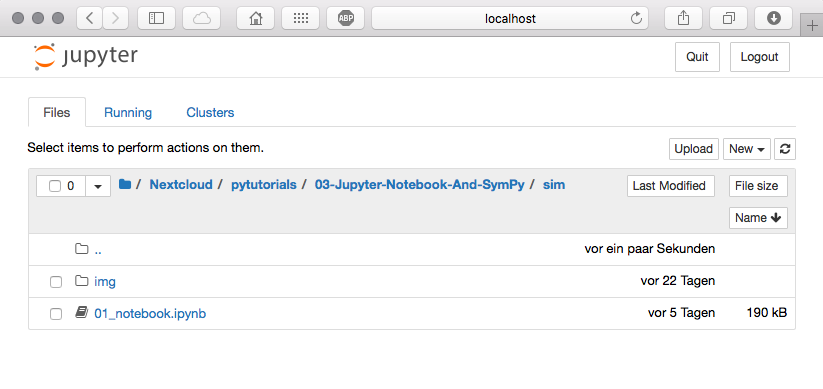
\includegraphics[scale=0.4]{img/jupyter_screenshot}
\end{figure}
\item Click on \texttt{01\_notebook.ipynb} to run the notebook or click on $\texttt{New}$ to create a new one.
\end{enumerate}  
\newpage
\section{SymPy}
\sympy is a \py library for symbolic mathematics. It enables the user to solve equation, integrals work in progress.
\subsection{Basic operations}

\end{document}

%%% Local Variables:
%%% mode: latex
%%% TeX-master: t
%%% End: